\documentclass[11pt, spanish, a4paper, twopage]{article}
% Versión 1.er cuat 2021 Víctor Bettachini < bettachini@df.uba.ar >

% Versión 1.er cuat 2021 Víctor Bettachini < bettachini@df.uba.ar >

\usepackage[T1]{fontenc}
\usepackage[utf8]{inputenc}

\usepackage[spanish, es-tabla]{babel}
\def\spanishoptions{argentina} % Was macht dass?
% \usepackage{babelbib}
% \selectbiblanguage{spanish}
% \addto\shorthandsspanish{\spanishdeactivate{~<>}}

\usepackage{graphicx}
\graphicspath{{./figuras/}{../LaTeX/}}
% \usepackage{float}

\usepackage[arrowdel]{physics}
\newcommand{\pvec}[1]{\vec{#1}\mkern2mu\vphantom{#1}}
% \usepackage{units}
\usepackage[separate-uncertainty=true, multi-part-units=single, locale=FR]{siunitx}
\usepackage{isotope} % $\isotope[A][Z]{X}\to\isotope[A-4][Z-2]{Y}+\isotope[4][2]{\alpha}

\usepackage{tasks}
\usepackage[inline]{enumitem}
% \usepackage{enumerate}

\usepackage{hyperref}

% \usepackage{amsmath}
% \usepackage{amstext}
\usepackage{amssymb}

\usepackage{tikz}
\usepackage{tikz-dimline}
\usetikzlibrary{calc}
% \usetikzlibrary{math}
\usetikzlibrary{arrows.meta}
\usetikzlibrary{snakes}
\usetikzlibrary{decorations}
\usetikzlibrary{decorations.pathmorphing}
\usetikzlibrary{patterns}

% \usepackage[hmargin=1cm, vmargin=1cm, includeheadfoot]{geometry}
\usepackage[hmargin=1cm,vmargin=3cm, top= 0.75cm,nohead]{geometry}
% \voffset-3.5cm
% \hoffset-3cm
% \setlength{\textwidth}{17.5cm}
% \setlength{\textheight}{27cm}

\usepackage{lastpage}
\usepackage{fancyhdr}
\pagestyle{fancyplain}
\fancyhf{}
% \fancyhead{}
\setlength\headheight{28.7pt} 
\fancyhead[LE, LO]{\textbf{Física 2} (Físicos) }
% \lhead{\textbf{Física 2} (Físicos) }
\fancyhead[RE, RO]{\href{https://df.uba.ar/es/}{$\vcenter{\hbox{
\includegraphics[height=1cm]{sin_texto.pdf}}}$}}
% \rhead{$\vcenter{\hbox{
\includegraphics[height=1cm]{sin_texto.jpg}}}$}
% \rhead{
\includegraphics[height=1cm]{sin_texto.jpg}}
% \rhead{\textcopyright {\tt DF, FCEyN, UBA}}
\fancyfoot{\href{https://creativecommons.org/licenses/by-sa/4.0/deed.es/}{$\vcenter{\hbox{
\includegraphics[height=0.4cm]{cc-by-sa.pdf}}}$} \href{https://df.uba.ar/es/}{DF, FCEyN, UBA}}
% \fancyfoot{$\vcenter{\hbox{
\includegraphics[height=0.4cm]{cc-by-sa.pdf}}}$ DF, FCEyN, UBA}
% \fancyfoot{{\tiny \textcopyright DF, FCEyN, UBA}}
\fancyfoot[C]{ {\tiny Actualizado al \today} }
\fancyfoot[RO, LE]{Pág. \thepage/\pageref{LastPage}}
\renewcommand{\headrulewidth}{0pt}
\renewcommand{\footrulewidth}{0pt}


\begin{document}
\begin{center}
% \textbf{Física 2} (Físicos) \hfill \textcopyright {\tt DF, FCEyN, UBA}\\
	\textsc{\LARGE Reflexión y transmisión de ondas}
\end{center}

Los ejercicios con (*) entrañan una dificultad adicional. Son para investigar después de resolver los demás.


\begin{enumerate}

\section*{Discontinuidades en cuerdas}


\item 
\begin{minipage}[t][1.6cm]{0.6\textwidth}
Nos interesa estudiar la unión de dos cuerdas de distinta densidad lineal $\lambda_{m1}$ y $\lambda_{m2}$, por lo que las consideraremos semi--infinitas. 
Mientras se las somete a una tensión constante, \(T_0\), incide desde la primera una onda $\psi_i(x,t) = A_i \cos{ \left( k_{1} x- \omega t \right) }$.
\end{minipage}
\begin{minipage}[c][-0.2cm][t]{0.34\textwidth}
	\begin{tikzpicture}[scale= 1]
		\draw [ultra thick, dashed] (-3,0) -- (-2,0);
		\draw [ultra thick] (-2,0) -- (0,0) node [near start, above] {\(\lambda_{m1} \)};
		\draw [thin] (0,0) -- (2,0) node [near end, above] {\(\lambda_{m2} \)}; % node [midway, above] {\(\lambda_{m2} \)};
		\draw [thin, dashed] (2,0) -- (3,0);
	\end{tikzpicture}
\end{minipage}
\begin{enumerate}
	\item Calcule $k_{1}$ y $k_{2}$, es decir, los números de onda a cada lado de la unión.
	\item Plantee la solución más general para $\psi(x,t)$ de cada lado de la unión.
	\item ¿Qué condiciones deben verificarse en el punto de unión de las cuerdas?
	\item Usando b) y c), calcule la perturbación $\psi(x,t)$ en cada una de las cuerdas.
	\item Determine coeficientes de reflexión, $R$, y transmisión, $T$.
	¿Qué sucede en el caso \(\lambda_{m2} \rightarrow \infty\)?
	¿Y sí \(\lambda_{m1} \to \lambda_{m2}\)? 
\end{enumerate}



\item 
\begin{minipage}[t][2.3cm]{0.6\textwidth}
La cuerda de la izquierda, de densidad \(\lambda_{m1}\) y largo \(L\), se encuentra fija en su extremo izquierdo a la pared, y en su extremo derecho a otra cuerda semi-infinita de densidad \(\lambda_{m2}\).
Todo el sistema se encuentra sometido a tensión \(T_0\).
Suponga que por la cuerda de densidad \(\lambda_{m2}\) incide la onda armónica \(\psi_i(x,t) = A_i \mathrm{e}^{i (\omega t + k_2 x) }\).
\end{minipage}
\begin{minipage}[c][0.2cm][t]{0.34\textwidth}
	\begin{tikzpicture}[scale= 1]
		\draw (-2,-1) -- (-2,1); % pared vertical
		\fill [pattern = north east lines] (-2.25,-1) rectangle (-2,1);
		\draw [ultra thick] (-2,0) -- (0,0) node [midway, above] {\(\lambda_{m1} \)};
		\draw [thin] (0,0) -- (3,0) node [midway, above] {\(\lambda_{m2} \)};
		\dimline [extension start length= -0.2, extension end length = -0.2] {(-2,-0.4)}{(0,-0.4)}{\(L\)}; 
		\draw [thin, dashed] (3,0) -- (4,0);
	\end{tikzpicture}
\end{minipage}
\begin{enumerate}
	\item Imponga las condiciones de contorno apropiadas y determine \(\psi(x,t)\) en cada sector de la cuerda.
	\item Halle los valores de \(L\) para los cuales hay un nodo de desplazamiento en la unión de las cuerdas.
\end{enumerate}


\item 
\begin{minipage}[t][1.6cm]{0.6\textwidth}
Una cuerda de densidad lineal \(\lambda_m\) sometida a una tensión \(T_0\) tiene en su centro, \(x= 0\), un pequeño nudo de masa \(M\).
Este causa que sea parcialmente reflejada viajando en la dirección de las \(x\) positivas dada por \(\psi_i(x,t) = A_i \mathrm{e}^{i ( k x - \omega t ) }\).
\end{minipage}
\begin{minipage}[c][-0.5cm][t]{0.34\textwidth}
	\begin{tikzpicture}[scale= 1]
		\draw [thick, dashed] (-3,0) -- (-2,0);
		\draw [thick] (-2,0) -- (0,0) node [near start, above] {\(\lambda_m \)};
		% \draw [thick] (-2,0) -- (2,0); % node [midway, above] {\(\lambda_{m2} \)};
		\draw [thick] (0,0) -- (2,0) node [near end, above] {\(\lambda_m \)};
		\draw [thick,dashed] (2,0) -- (3,0);
		\shade [ball color=black!80] (0,0) circle(0.25) node [] {\color{white} $M$};
	\end{tikzpicture}
\end{minipage}
\begin{enumerate}
	\item Plantee la solución más general para la onda \(\psi (x,t)\) a cada lado del nudo,
	\item y las condiciones de empalme.
	Demuestre que una condición le permite definir que \(A_i + A_r = A_t\) y que la otra implica que \(A_i - A_r = (1 + i \frac{M \omega^2}{k T} )A_t\).
\end{enumerate}



\section*{Interfaces para el sonido}

\item
\begin{minipage}[t][2.8cm]{0.6\textwidth}
Como nos interesa estudiar la unión de dos caños cuadrados de área transversal $A_1$ y $A_2$ los consideramos semi--infinitos.
Desde el izquierdo incide una onda acústica $\delta p_i (x,t) = a_i \cos{ \left( k_i x - \omega t \right) }$.
Suponga despreciables los efectos de la viscosidad y dé por conocidos $A_{1}$, $A_{2}$, presión media $P_{0}$, densidad media $\rho_{0}$, $v_{s}$, $\omega$, $a_i$.
Halle amplitudes de presión y desplazamiento de moléculas a causa de las ondas reflejadas y transmitidas.
\end{minipage}
\begin{minipage}[c][0cm][t]{0.34\textwidth}
	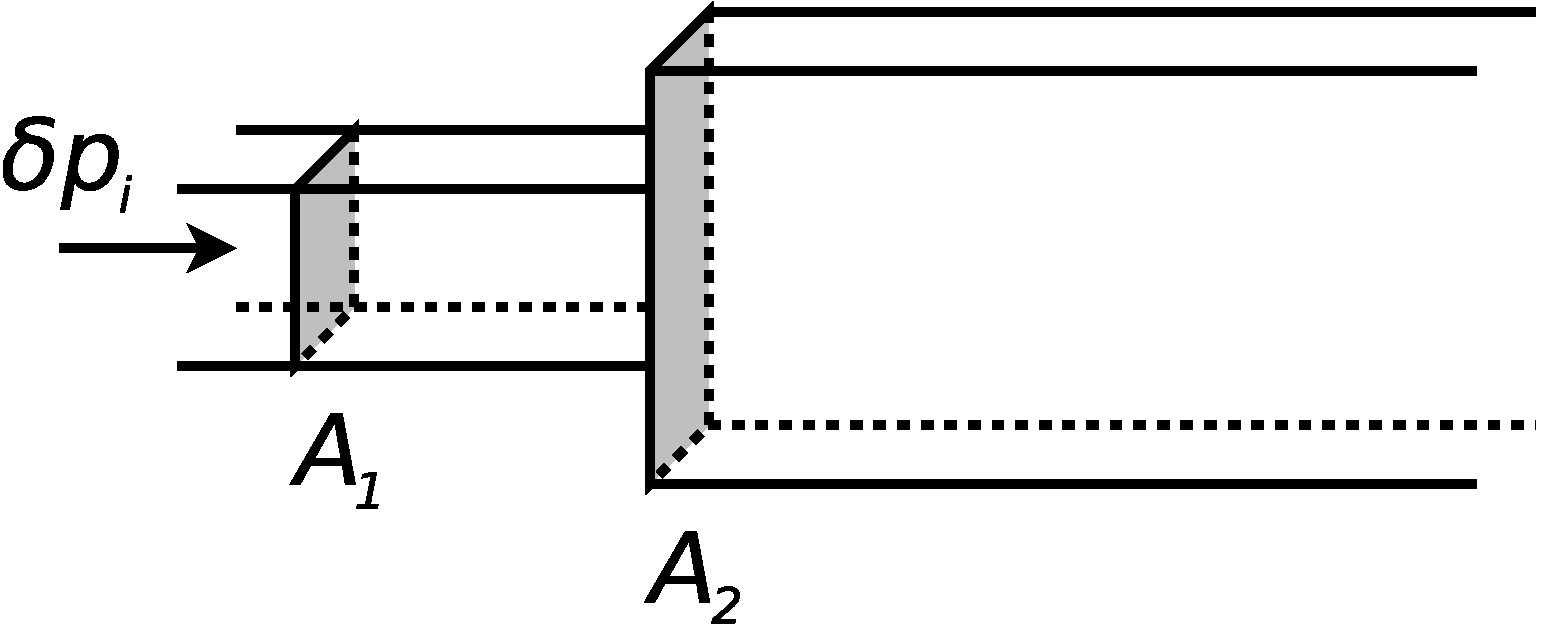
\includegraphics[width=\textwidth]{ej2-10}
\end{minipage}



\item 
\begin{minipage}[t][1.4cm]{0.6\textwidth}
A este armado con idénticas áreas del problema anterior incide la misma onda.
Halle $\delta p(x,t)$ y $\psi(x,t)$ en cada tramo.
\end{minipage}
\begin{minipage}[c][1.4cm][t]{0.34\textwidth}
	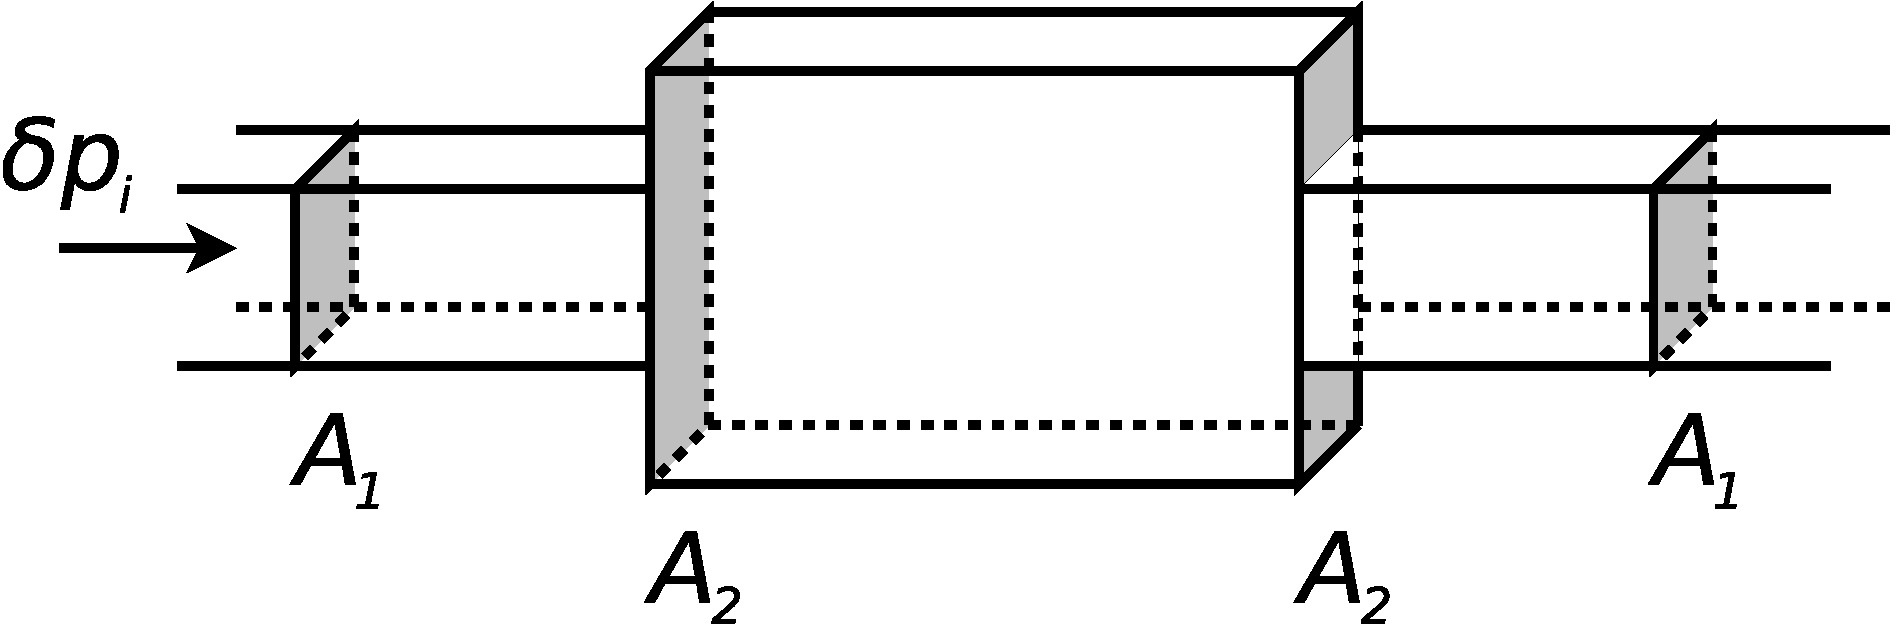
\includegraphics[width=\textwidth]{ej2-11}
\end{minipage}



\item
\begin{minipage}[t][1.6cm]{0.75\textwidth}
(*) Desde el aire incide en dirección perpendicular a una superficie calma de agua una onda de sonido plana $\delta p_i (y,t) = A_i \cos{\left( k_i y - \omega t \right)}$.
Hallar la onda reflejada $\delta p_{r}(y,t)$ y transmitida $\delta p_{t}(y,t)$.
\end{minipage}
\begin{minipage}[c][0.8cm][t]{0.2\textwidth}
	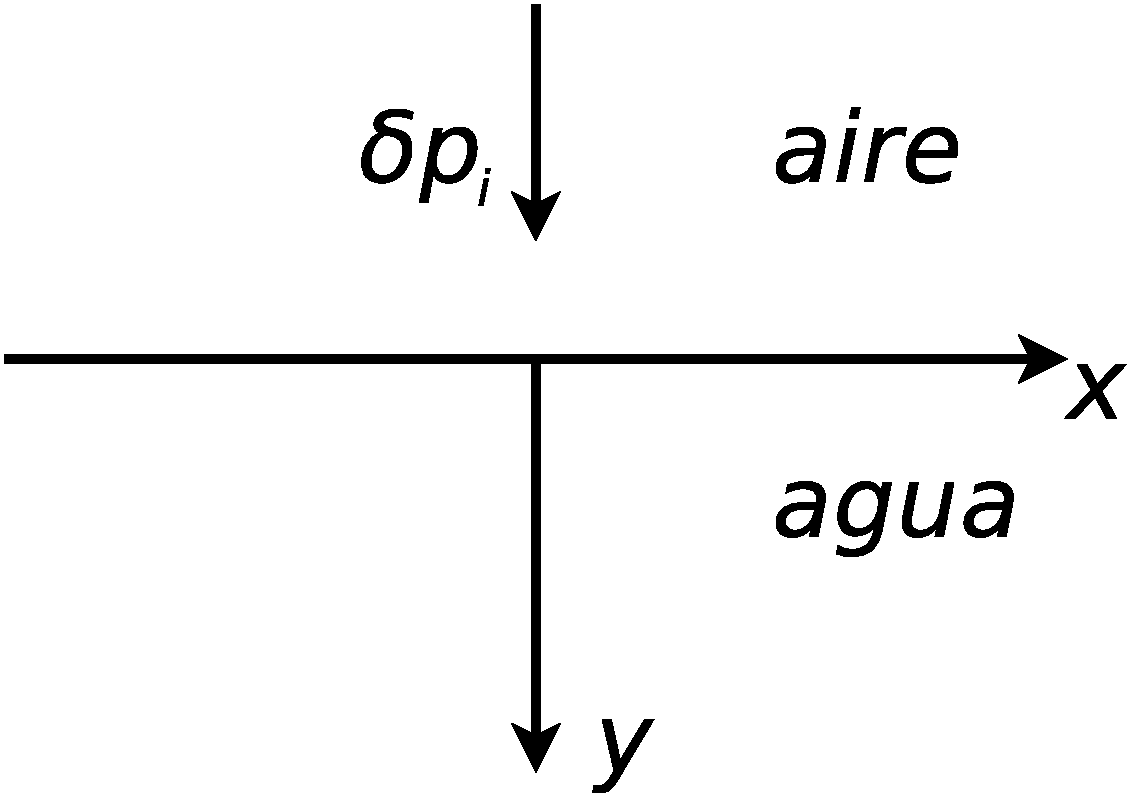
\includegraphics[width=\textwidth]{ej2-12}
\end{minipage}
%\begin{figure}[ht]
%\centering{}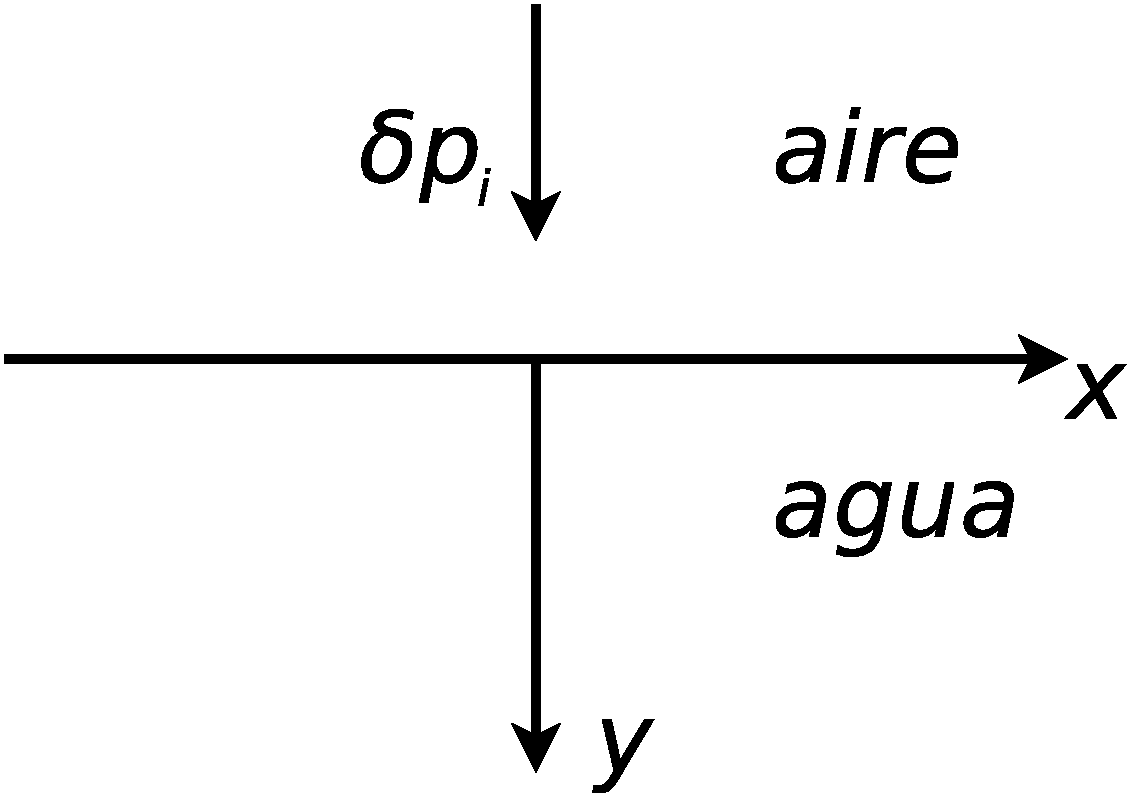
\includegraphics[clip,scale=0.25]{ej2-12}
%\end{figure}


\item (*)
Calcule los coeficientes de reflexión y de transmisión del sonido en las siguientes interfases:\\
\begin{enumerate*}[label=\alph*),itemjoin={,\quad}]
	\item Fe-Cu
	\item Al-Pb
\end{enumerate*}
%\begin{enumerate}
%	\item Fe-Cu
%	\item Al-Pb
%\end{enumerate}


\end{enumerate}

\end{document}



\end{enumerate}

\end{document}
